%%%%%%%%%%%%%%%%%%%%%%%%%%%%%%%%%%%%%%%%%
% University/School Laboratory Report
% LaTeX Template
% Version 3.1 (25/3/14)
%
% This template has been downloaded from:
% http://www.LaTeXTemplates.com
%
% Original author:
% Linux and Unix Users Group at Virginia Tech Wiki 
% (https://vtluug.org/wiki/Example_LaTeX_chem_lab_report)
%
% License:
% CC BY-NC-SA 3.0 (http://creativecommons.org/licenses/by-nc-sa/3.0/)
%
%%%%%%%%%%%%%%%%%%%%%%%%%%%%%%%%%%%%%%%%%

%----------------------------------------------------------------------------------------
%	PACKAGES AND DOCUMENT CONFIGURATIONS
%----------------------------------------------------------------------------------------

\documentclass{article}

\usepackage[version=3]{mhchem} % Package for chemical equation typesetting
\usepackage{siunitx} % Provides the \SI{}{} and \si{} command for typesetting SI units
\usepackage{graphicx} % Required for the inclusion of images
\usepackage{natbib} % Required to change bibliography style to APA
\usepackage{amsmath} % Required for some math elements 
\usepackage[utf8]{inputenc}
\usepackage[margin=1.2in]{geometry}

\setlength\parindent{0pt} % Removes all indentation from paragraphs

% \renewcommand{\labelenumi}{\alph{enumi}.} % Make numbering in the enumerate environment by letter rather than number (e.g. section 6)

\renewcommand{\figurename}{Figura}
\renewcommand{\tablename}{Tabla}
\renewcommand\refname{Referencias}

%\usepackage{times} % Uncomment to use the Times New Roman font

%----------------------------------------------------------------------------------------
%	DOCUMENT INFORMATION
%----------------------------------------------------------------------------------------

\title{M\'etodos num\'ericos para la Ciencia e Ingenier\'ia \\ Tarea 6: Ecuaciones de reacción-difusión} % Title

\author{Felipe Toledo Bittner} % Author name

\date{\today} % Date for the report

\begin{document}

\maketitle % Insert the title, author and date

%----------------------------------------------------------------------------------------
%	SECTION 1
%----------------------------------------------------------------------------------------

\section{Introducción}

Los sistemas de reacción-difusión se utilizan para modelar matemáticamente fenómenos espaciales en que el valor de una variable en cada punto presenta dependencia tanto de reacciones locales como de difusión desde los puntos cercanos. Su forma general puede verse en la ecuación (\ref{eq:reaccion_difusion}). El primer término de la derecha corresponde a la componente difusiva y el segundo a la reactiva, en este caso modelada como el polinomio $P(n)$.

\begin{equation}
  \dfrac{dn}{dt} = \gamma \dfrac{d^2n}{dx^2} + P(n)
  \label{eq:reaccion_difusion}
\end{equation}

En este trabajo se implementa una clase en python que permite crear un sistema de reacción-difusión unidimensional y resolverlo para un intervalo de tiempo escogido por el usuario. Se incluyen métodos que permiten setear la variable $\gamma$, los coeficientes del polinomio $P(n)$ y las condiciones iniciales y de borde.

\section{Descripción de la solución}

La clase implementada permite resolver cualquier sistema de reacción-difusión que posea la forma de la ecuación (\ref{eq:reaccion_difusion}). En el archivo \emph{main\_p1.py} adjunto a este informe hay un ejemplo bien comentado con los pasos a seguir para inicializar el programa, en este caso con la ecuación de Fisher-KPP.
 
\subsection{Algoritmo de integración}
\label{sec:algoritmo_integracion}

Para integrar la ecuación de forma numérica se opta por utilizar dos métodos, Crank-Nicolson para la parte de difusión y una versión modificada del método de Euler para la de reacción. La modificación ha sido una elaboración propia, y es justificada a continuación.

Inicialmente consideremos el caso en que no hay componente de difusión. La ecuación (\ref{eq:reaccion_difusion}) queda escrita en forma numérica como se muestra en (\ref{eq:no_difusion}). Los subíndices $(x,t)$ en este caso representan posiciones y tiempos discretos y $h$ es el paso temporal de la integración.

\begin{equation}
  \frac{n_{x,t+1} - n_{x,t}}{h} = P(n_{x,y})
  \label{eq:no_difusion}
\end{equation} 

Que se puede integrar usando el método de Euler, como se indica en la ecuación (\ref{eq:metodo_euler}). Se observa que el lado derecho consiste simplemente en la actualización de la variable $n$ usando su pendiente en cada instante de tiempo. Apartemos esto un momento para estudiar la parte difusiva, pero no debemos olvidarlo aún.

\begin{equation}
  n_{x,t+1}^e = n_{x,t} + h P(n_{x,t})
  \label{eq:metodo_euler}
\end{equation}

Suponiendo ahora que sólo hay componente difusiva, la ecuación original puede escribirse como (\ref{eq:no_reaccion}). Aquí se utiliza el promedio entre las segundas derivadas calculadas hacia adelante y atrás para aproximar mejor el cambio en $n$.

\begin{equation}
  \frac{n_{x,t+1} - n_{x,t}}{h} = \frac{1}{2} \left( \frac{n_{x+1,t+1} - 2 n_{x,t+1} + n_{x-1,t+1} }{h^2} + \frac{n_{x+1,t} - 2 n_{x,t} + n_{x-1,t} }{h^2} \right)
  \label{eq:no_reaccion}
\end{equation}

A partir de aquí se puede plantear un sistema de ecuaciones lineales para encontrar el valor de los $n_{x,t+1}$ desconocidos a partir de los $n_{x,t}$ conocidos para todos los puntos $x$ simultáneamente. Éste es el llamado método de Crank-Nicolson, explicado en múltiples excelentes referencias \footnote{Por ejemplo el documento "Solucion Numerica de la Ecuacion de Calor por el Metodo de las Diferencias Finitas", realizado por Miguel Caro C. del Departamento de Matematicas de la Universidad del Atlantico de Colombia, entre otros. Puede encontrarse en línea en el sitio http://www.icmc.usp.br/CMS/Arquivos/arquivos\_enviados/BIBLIOTECA\_113\_RT\_327.pdf}.

El resultado de esta operación calcula todos los $n_{x,t+1}$. A grandes rasgos el resultado de una iteración puede describirse como se ve en la ecuación (\ref{eq:actualizacion_nicolson}), donde $CN( \Delta x, h, \mathbf{n} )$ es el término de actualización, $\Delta x$ la distancia entre puntos en unidades de longitud físicas y $\mathbf{n}$ el vector que contiene todos los $n_{x,t}$.

\begin{equation}
  n_{x,t+1}^{cn} = n_{x,t} + CN( \Delta x, h, \mathbf{n} )
  \label{eq:actualizacion_nicolson}
\end{equation} 

En principio, calcular el valor completo de $n_{x,t+1}$ debiese ser tan sencillo como sumar $n_{x,t+1} = n_{x,t+1}^{cn} + n_{x,t+1}^{e}$, pero al hacer esto aparece un problema. Como se ve en la ecuación (\ref{eq:solucion_mala}), al hacer esta operación aparece un término $2n_{x,t}$. Este término es espurio y debe corregirse ya que el espíritu de la integración numérica es ir actualizando $n_{x,t}$ usando sus tasas de cambio, dadas en este caso por $CN(...)$ y $P(n)$. 

\begin{equation}
  n_{x,t+1} = n_{x,t+1}^{cn} + n_{x,t+1}^{e} = \mathbf{2n_{x,t}} + CN( \Delta x, h, \mathbf{n} ) + h P(n_{x,t})
  \label{eq:solucion_mala}
\end{equation}

Para corregir el inconveniente, se opta por modificar el método de euler, dejándolo de la forma $n_{x,t+1}^{e^*} = h P(n_{x,t})$. Tras esta modificación, la ecuación (\ref{eq:solucion_mala}) toma la forma (\ref{eq:solucion_buena}), que como se ve en secciones posteriores logra integrar correctamente el sistema de difusión-reacción.

\begin{equation}
  n_{x,t+1} = n_{x,t+1}^{cn} + n_{x,t+1}^{e^*} = n_{x,t} + CN( \Delta x, h, \mathbf{n} ) + h P(n_{x,t})
\label{eq:solucion_buena}
\end{equation}

\section{Resultados}

\subsection{Caso 1}

En este caso se modela un sistema de Fisher-KPP, el cual consiste en la siguiente ecuación:

\begin{equation}
  \frac{\partial n}{\partial t} = \gamma \frac{\partial^2n}{\partial x^2} + \mu n - \mu n^2
  \label{Fisher-KPP}
\end{equation}

En este caso $n$ representa la densidad de una especie en función del tiempo y la posición. Los parámetros usados son:

\begin{enumerate}
  \item Largo de 1 [m]
  \item Discretizado de 500 puntos
  \item $\gamma$ = 0.001
  \item $\mu  = 1.5$
  \item Resolución: $h = 0.001$[s], $\Delta x = 0.002$[m]
  \item Condiciones de borde: $n(t, x=0) = 1$ y $n(t, x=1) = 0$
  \item Condiciones iniciales: $ n(0, x) = e^{-x^2/0.1} $
  \item Tiempo final de integración: $t_f = 4[s]$
\end{enumerate}

Tras integrar la ecuación para 4 segundos, se obtienen los resultados de la siguiente figura:

\begin{figure}[ht]
  \centering
  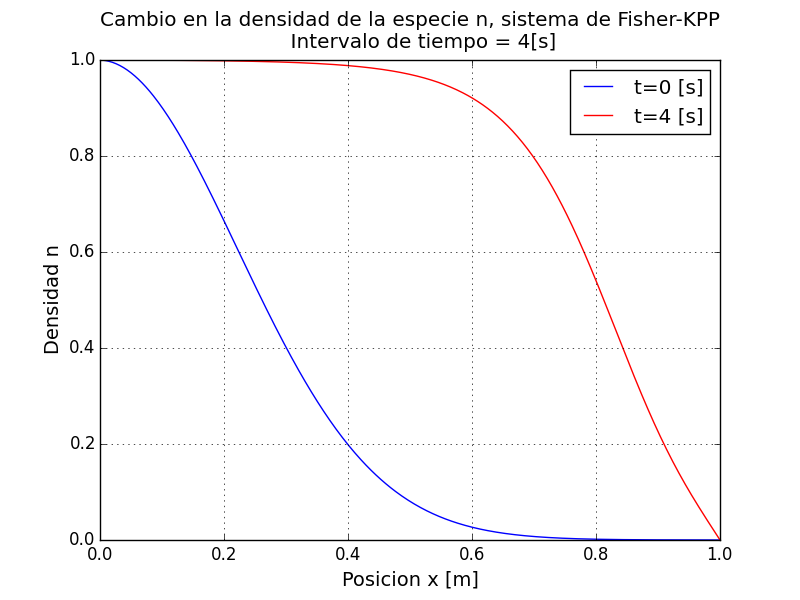
\includegraphics[scale = 0.55]{images/resultados_p1.png}
  \label{fig:resultados_p1}
  \caption{Resultados de la integración de la ecuación de Fisher-KPP.}
\end{figure}

Se observa que la densidad comienza a aumentar hacia la derecha con el paso del tiempo. Una forma de entender esto es viendo la condición de borde izquierda como una fuente de densidad, la que intenta difundir hacia la derecha generando una ola. A medida que nos alejamos de la fuente, comienza a dominar el término de reacción de competencia ($-\mu n^2$), acotando los máximos valores de $n$ llegando a 0 en el extremo derecho debido a la otra condición de borde.

\subsection{Caso 2}

Ahora se integra la ecuación de Newell-Whitehead-Segel:

\begin{equation}
  \frac{\partial n}{\partial t} = \gamma \frac{\partial^2n}{\partial x^2} + \mu ( n - n^3 )
\end{equation}

Usando las siguientes condiciones:

\begin{enumerate}
  \item Largo de 1 [m]
  \item Discretizado de 500 puntos
  \item $\gamma$ = 0.001
  \item $\mu  = 1.5$
  \item Resolución: $h = 0.001$[s], $\Delta x = 0.002$[m]
  \item Condiciones de borde: $n(t, x=0) = 0$ y $n(t, x=1) = 0$
  \item Condiciones iniciales: $ n(0, x) = random(-0.3,0.3) $
  \item Tiempo final de integración: $t_f = 4[s]$
\end{enumerate}

En este caso se resuelve para dos conjuntos de condiciones iniciales donde cada n toma un valor aleatorio entre -0.3 y 0.3, generado usando la función \emph{random.uniform()} de numpy. Con el fin de obtener resultados replicables se establecen dos semillas $s1 = 317$ y $s2 = 119$ con la función \emph{random.seed(<int>)} de la misma librería.

Los resultados se presentan en la figura a continuación:

\begin{figure}[ht]
  \centering
  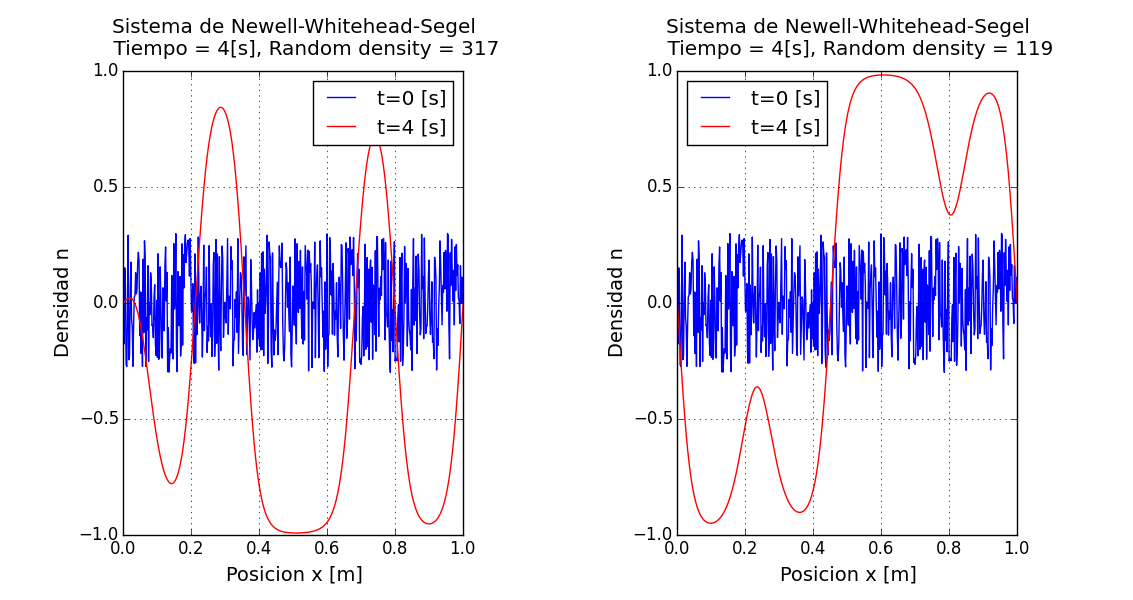
\includegraphics[scale = 0.55]{images/resultados_p2.png}
  \label{fig:resultados_p2}
  \caption{Resultados de la integración de la ecuación de Newell-Whitehead-Segel para dos condiciones iniciales distintas.}
\end{figure}

De las figuras se puede apreciar que la diferencia en las condiciones iniciales genera resultados completamente distintos tras el período de cálculo, lo que puede explicarse argumentando que se está integrando cerca de un punto de equilibrio inestable. El respaldo de esta afirmación proviene de que los valores aleatorios están acotados entre [-0.3, 0.3], por lo que se comienza a resolver desde puntos más cercanos a $0$ (punto de equilibrio inestable) que a $\pm 1$ (puntos de equilibrio estable).

\section{Conclusiones}

El principal logro de esta tarea es que se logra implementar código que permite trabajar con sistemas de difusión-reacción de forma general, operando además bajo el paradigma de programación orientada a objetos. Esto, junto a la documentación aquí presentada, los comentarios en el código y los ejemplos desarrollados debiese permitir a cualquier otra persona usar este código de forma explícita o encapsulada para resolver sus propios sistemas de difusión-reacción en una dimensión.

También se concluye que al utilizar varios métodos simultáneos de integración numérica se debe considerar su interacción para no obtener elementos redundantes en el cálculo, como se vió en la sección \ref{sec:algoritmo_integracion}

Para el trabajo futuro se propone implementar optimizaciones de forma consciente en el código para disminuir el tiempo de cálculo de las rutinas más pesadas. Para este caso particular, por ejemplo, sería recomendable mejorar la velocidad del algoritmo de Crank-Nicolson, ya que es iterado muchas veces y toma un tiempo mayor que las otras rutinas debido a que realiza operaciones con matrices (inversión y multiplicación).

\end{document}
